\begin{frame}[noframenumbering,plain]
    \setcounter{framenumber}{1}
    \maketitle
\end{frame}

\begin{frame}{Беспилотные транспортные средства}
	Последние десятилетия характеризуются активным внедрением и распро­странением беспилотных транспортных средств (далее \textbf{БТС}) в различных сферах человеческой деятельности:
	\begin{itemize}
		\item логистика, промышленность,
		\item сельское хозяйство, горное дело,
		\item городская инфраструктура.
	\end{itemize}
	\centering
	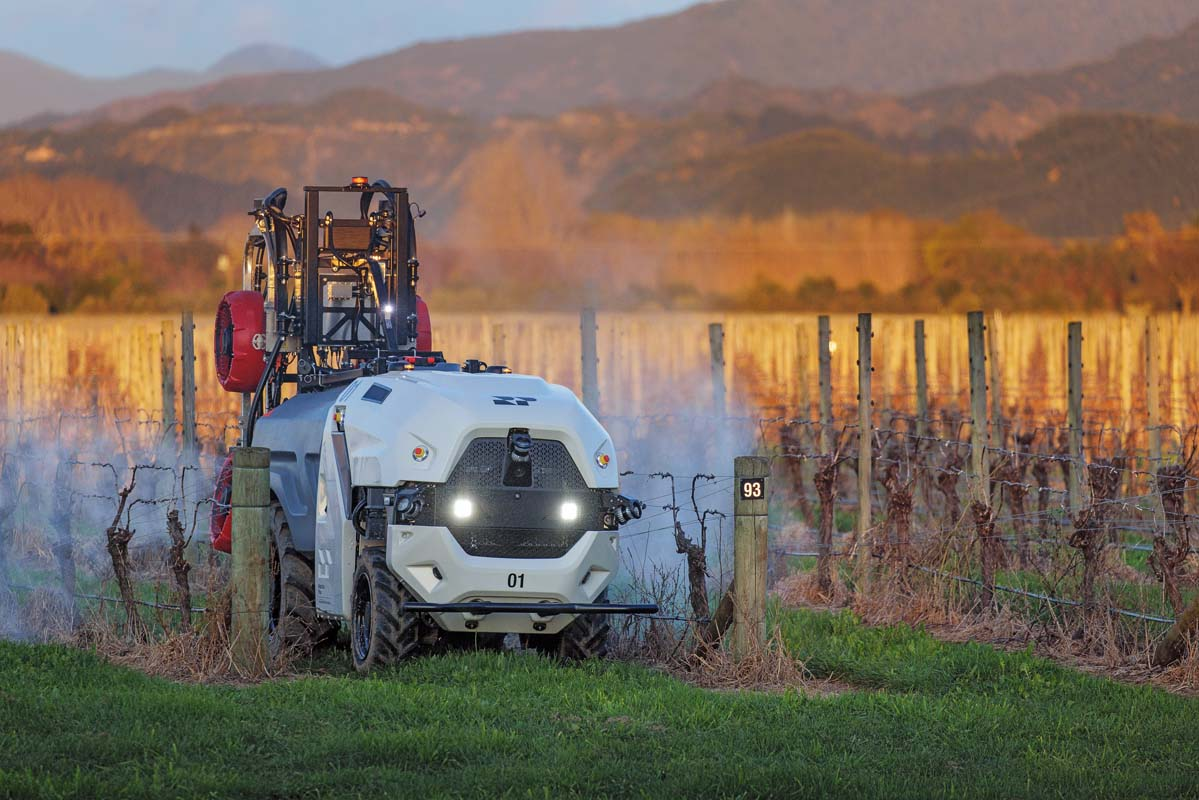
\includegraphics[width=0.3\linewidth]{Presentation/images/usage_1}
	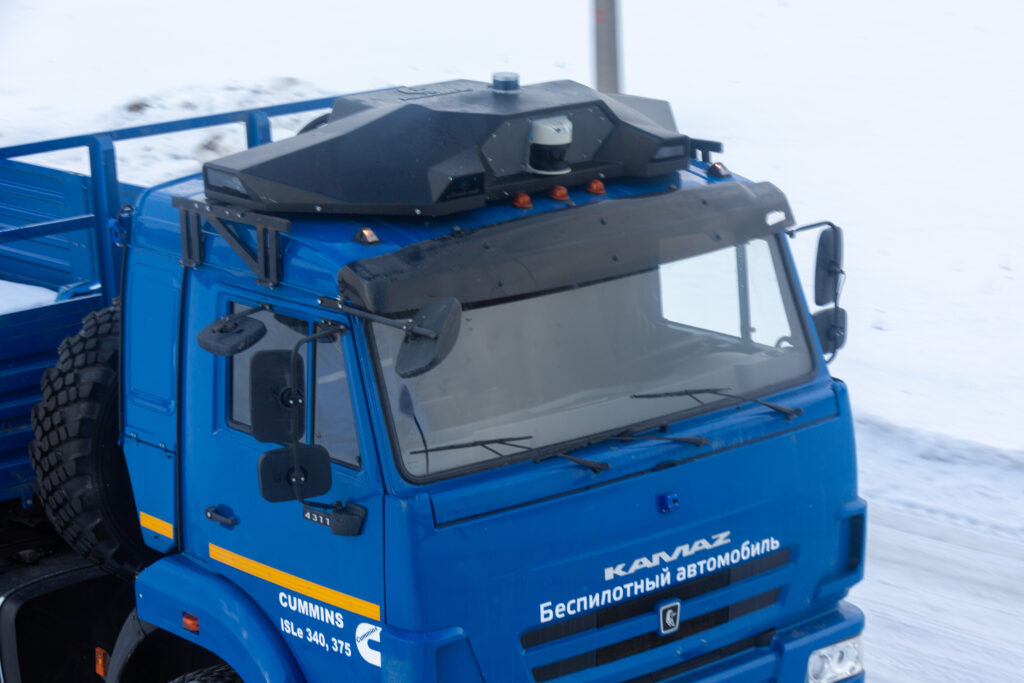
\includegraphics[width=0.3\linewidth]{Presentation/images/usage_2}
	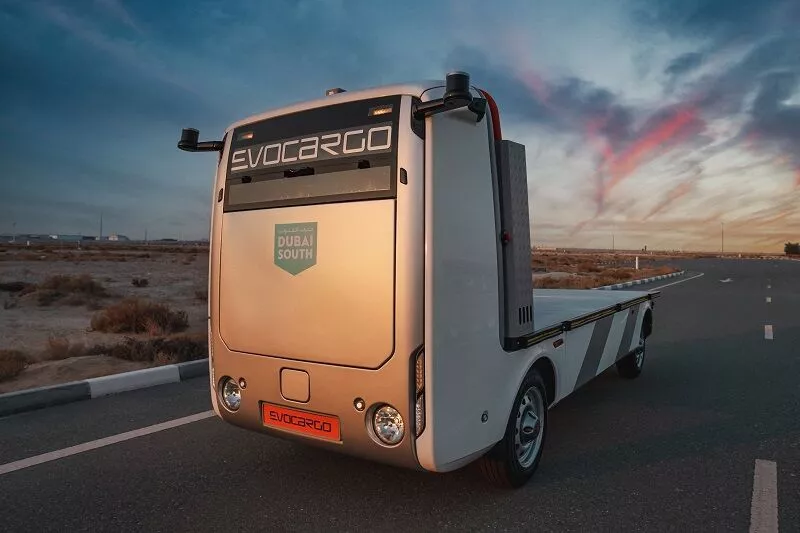
\includegraphics[width=0.3\linewidth]{Presentation/images/usage_3}\\
	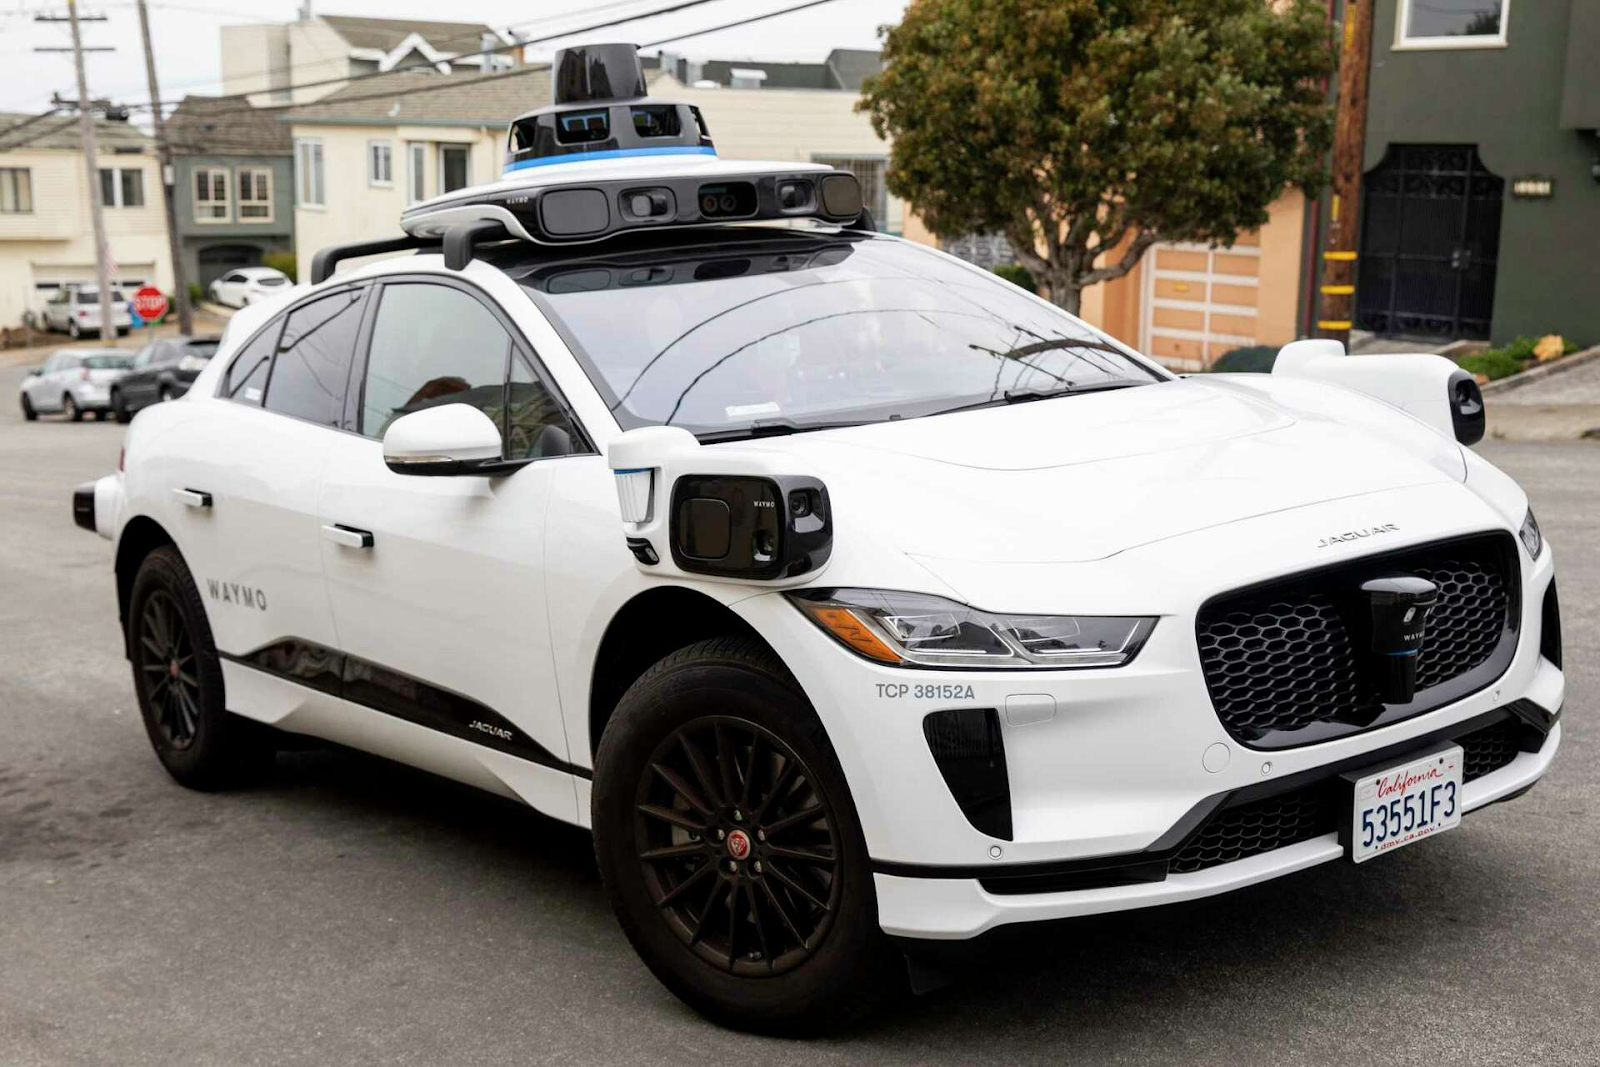
\includegraphics[width=0.3\linewidth]{Presentation/images/usage_4}
	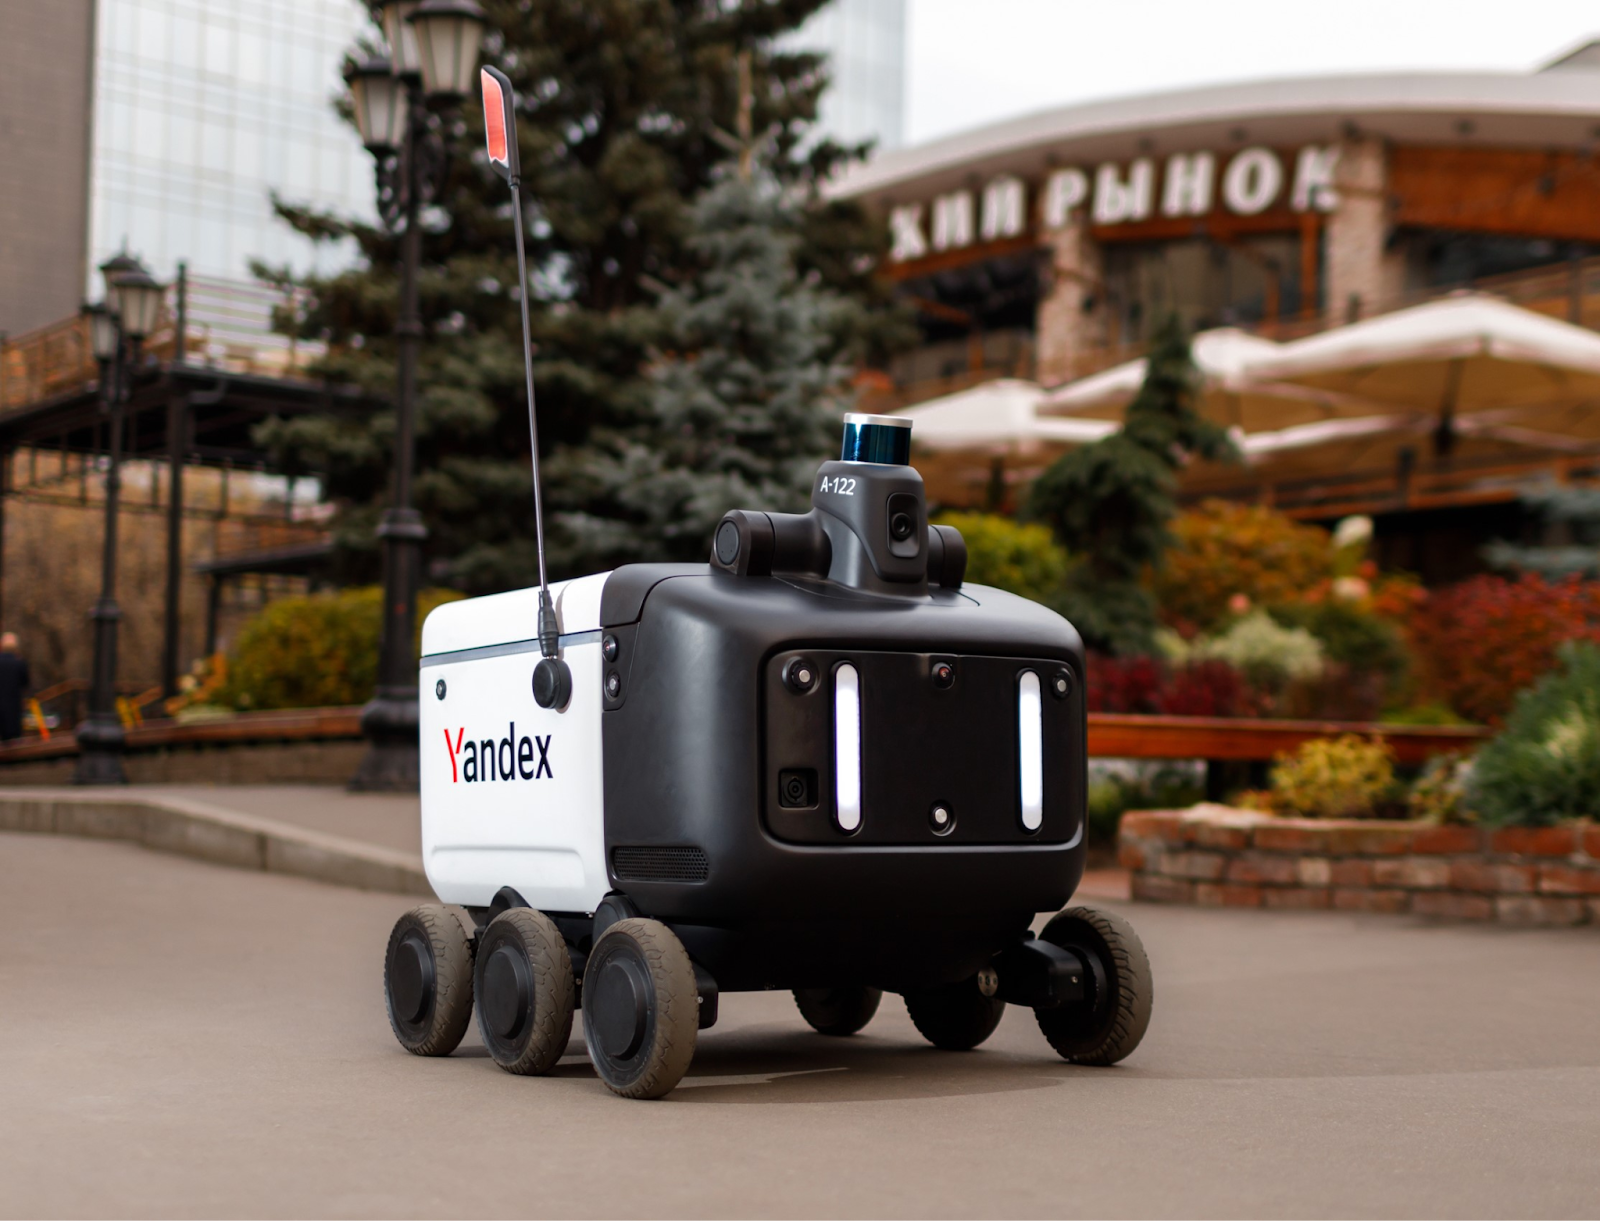
\includegraphics[width=0.3\linewidth]{Presentation/images/usage_5}\\
\end{frame}
\note{
    Развитие беспилотного транспорта входит в перечень критических технологий РФ;
    Транспортная стратегия РФ до 2030 года включает движение БТС по дорогам общего пользования.
}

\begin{frame}{Основные программные компоненты БТС}
	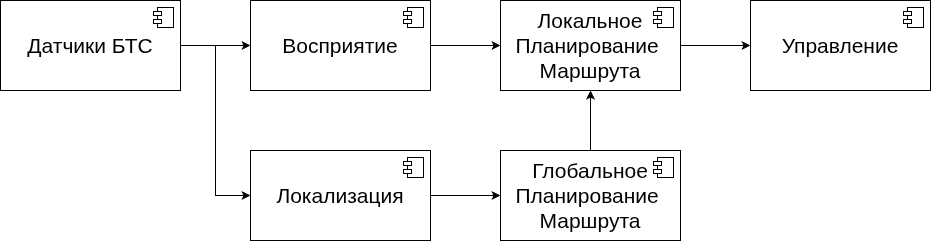
\includegraphics[width=\linewidth]{Presentation/images/AV_components}
\end{frame}

\begin{frame}{Модель окружающего пространства}
	Для планирования безопасного маршрута БТС требуется \textbf{модель окружающего пространства}. Требования к модели:

	\begin{itemize}
		\item степень детализации описания пространства,
		\item вычислительная сложность построения модели,
		\item объём занимаемой памяти вычислителя.
	\end{itemize}

	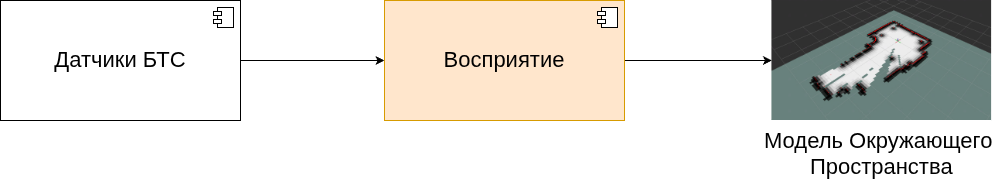
\includegraphics[width=\linewidth]{Presentation/images/PerceptionTask.drawio}
\end{frame}

\begin{frame}{Датчики БТС}
	\footnotesize
	Модель строится по измерениям бортовых датчиков. Каждый тип датчика обладает своими преимуществами и ограничениями\footnote{\fontsize{6}{7}\selectfont An overview of autonomous vehicles sensors and their vulnerability to weather conditions [Текст] / J. Vargas [и др.] // Sensors. --- 2021. --- Т.~21, №~16. --- С.~5397.}:

	\begin{table}
		\small
		\centering
		\begin{tabular}{|p{0.3\linewidth}|c|c|c|c|}
			\hline
			\textbf{Характеристика}          & \textbf{Лидар} & \textbf{Радар} & \textbf{Камера} & \textbf{Сонар}\\
			\hline
			\hline
			Разрешение                       & \cellcolor{yellow!25}Среднее & \cellcolor{red!25}Низкое  & \cellcolor{green!25}Высокое & \cellcolor{red!25}Низкое  \\
			\hline
			Дальность области обзора         & \cellcolor{yellow!25}150~м   & \cellcolor{green!25}250~м   & \cellcolor{yellow!25}200~м   & \cellcolor{red!25}5~м    \\
			\hline
			Устойчивость к погодным условиям & \cellcolor{yellow!25}Средняя & \cellcolor{green!25}Высокая & \cellcolor{red!25}Низкая  & \cellcolor{green!25}Высокая \\
			\hline
			Чувствительность к условиям освещения & \cellcolor{green!25}Нет & \cellcolor{green!25}Нет     & \cellcolor{red!25}Высокая & \cellcolor{green!25}Нет     \\
			\hline
			Информация о дистанции           & \cellcolor{green!25}Да      & \cellcolor{green!25}Да      & \cellcolor{red!25}Нет     & \cellcolor{green!25}Да      \\
			\hline
			Вычислительная нагрузка обработки & \cellcolor{yellow!25}Средняя & \cellcolor{green!25}Низкая & \cellcolor{red!25}Высокая & \cellcolor{green!25}Низкая  \\
			\hline
			Стоимость                        & \cellcolor{red!25}Высокая   & \cellcolor{yellow!25}Средняя & \cellcolor{green!25}Низкая  & \cellcolor{green!25}Низкая  \\
			\hline
		\end{tabular}
	\end{table}
\end{frame}

\begin{frame}{Комплексирование данных}
	\begin{itemize}
		\item Использование нескольких датчиков разных типов позволяет компенсировать ограничения отдельных датчиков и повысить качество модели.
		\item Задача объединения данных для определения текущего состояния объекта --- \textbf{задача комплексирования данных}.
		\item Наблюдается тренд на увеличение числа датчиков на БТС\footnote{\fontsize{6}{7}\selectfont Guerrero-Ibáñez J., Zeadally S., Contreras-Castillo J. Sensor Technologies for Intelligent Transportation Systems // Sensors. --- 2018.}.
	\end{itemize}

	\vfill
	По характеру взаимодействия комплексируемых данных\footnote{\fontsize{6}{7}\selectfont Durrant-Whyte H.~F. Sensor models and multisensor integration // The International Journal of Robotics Research. --- 1988.} выделяют:
	\begin{itemize}
		\item \textbf{конкурирующее} --- источники оценивают одно и то же свойство;
		\item \textbf{дополняющее} --- источники описывают разные свойства;
		\item \textbf{кооперативное} --- свойство недоступно ни одному источнику по отдельности.
	\end{itemize}
\end{frame}

\begin{frame}{Цена роста числа источников данных}
	\footnotesize
	Каждый источник увеличивает задержку между регистрацией данных и их учётом в модели. Размер карты определяется требованием безопасной остановки:
	\begin{columns}[T]
		\begin{column}{0.48\linewidth}
			$$v_{max} < \sqrt{2aR},\qquad N = \left(2R/res\right)^2 \Rightarrow N \propto v_{max}^4$$
		\end{column}
		\begin{column}{0.48\linewidth}
			$$S\,T(N) \le 1/f \Rightarrow \dfrac{S_{max}(v_2)}{S_{max}(v_1)} = \left(\dfrac{v_1}{v_2}\right)^{4}$$
		\end{column}
	\end{columns}

	\begin{table}
		\centering
		\resizebox{\textwidth}{!}{%
			\begin{tabular}{|l|c|c|c|c|}
				\hline
				\textbf{Рабочая скорость БТС $v_{max}$} & \textbf{20 км/ч} & \textbf{40 км/ч} & \textbf{60 км/ч} & \textbf{80 км/ч} \\ \hline
				Расстояние до границы карты $R$, м & $7,7$ & $30,9$ & $69,4$ & $123,5$ \\
				Размер карты $N$ (относительно 40 км/ч) & $-93,75$~\% & $1$ & $+406$~\% & $+1500$~\% \\
				Число источников $S_{max}$ (относительно 40 км/ч) & $+1500$~\% & $1$ & $-80,25$~\% & $-93,75$~\% \\ \hline
			\end{tabular}%
		}
	\end{table}

	\begin{itemize}
		\item При $40$~км/ч ($600\times600$ клеток, $T(N)\approx3$~мс, $f=10$~Гц) --- порядка трёх десятков источников.
		\item При $80$~км/ч --- лишь \textbf{два} источника данных.
	\end{itemize}
\end{frame}
\note{
    Отсюда --- требование к возможности одновременного обновления модели несколькими источниками.
}

\begin{frame}{Цель и задачи исследования}
	\footnotesize
	\textbf{Целью} данной работы является разработка методов построения моделей, описывающих проходимость окружающего пространства, предназначенных для работы на бортовом вычислителе БТС, обладающем ограниченными вычислительными ресурсами, в режиме реального времени и способных единовременно обрабатывать данные с большого количества бортовых датчиков, для повышения качества и актуальности модели окружающего пространства.

	Для достижения поставленной цели необходимо было решить следующие \textbf{задачи}:
	\begin{enumerate}
		\item Провести обзор существующих моделей окружающего пространства БТС и алгоритмов их построения для выбора базовой модели, описывающей проходимость пространства, и алгоритма её построения, которые будут использованы при разработке дальнейших алгоритмов.
		\item Разработать алгоритмы оценки положения объектов в окружающем пространстве БТС, а также областей проезжей части, доступных для движения БТС, на основе визуальных и лидарных данных, предназначенные для работы на бортовом вычислителе БТС в режиме реального времени.
		\item Разработать программный комплекс, обеспечивающий построение модели окружающего пространства БТС на основе комплексирования разнородных данных с бортовых датчиков БТС.
		\item Разработать структуру данных для представления модели окружающего пространства и параллельный алгоритм её обновления несколькими источниками данных.
	\end{enumerate}
\end{frame}

\begin{frame}[allowframebreaks]
    \frametitle{Положения, выносимые на защиту}
    \fontsize{8.5}{10.2}\selectfont
    \begin{enumerate}
    	\item Предложенный алгоритм вписывания проекции объекта на виде сверху в ориентированную ограничивающую рамку, опирающийся на модель L-образной формы видимой границы ТС, обеспечивает прирост среднего коэффициента Жаккара оценки положения окружающих ТС относительно сравниваемых общеизвестных алгоритмов, не использующих нейросетевые алгоритмы для вписывания проекции: $0,337$ против $0,328$ у лучшего из них (прирост $2,7$~\%).
    	\item Среди алгоритмов оценки положения объектов на плоскости движения БТС, применимых на бортовом вычислителе БТС в режиме реального времени, предложенный алгоритм комплексирования визуальных и лидарных данных, не использующий приближение поверхности дороги плоскостью, обеспечивает наибольший средний коэффициент Жаккара: прирост $10,0$~\% по сравнению с алгоритмом, использующим только лидарные данные ($0,439$ против $0,399$), и прирост $30,3$~\% по сравнению с алгоритмом, использующим только визуальные данные ($0,439$ против $0,337$).
    	\item Предложенный алгоритм проекции семантической сегментации проезжей части на плоскость движения БТС на основе комплексирования визуальных и лидарных данных в сочетании с базовым лидарным алгоритмом построения карты проходимости пространства повышает её качество по сравнению с картой, строящейся исключительно по лидарным данным: среднеквадратичная ошибка относительно эталонной карты снижается с $0,231$ до $0,218$ (на $5,6$~\%), а среднеквадратичная ошибка стоимости поиска пути (PathFinding Cost Mean Squared Error, PFC-MSE) --- с $1019,3$ до $924,4$ (на $9,3$~\%).
    	\item Предложенные структура данных для представления карты проходимости пространства и алгоритм, допускающий неблокирующее выполнение операций над картой, в одномерном случае уменьшают константу линейной вычислительной сложности цикла публикации карты в $13,89$ раза по сравнению с базовой реализацией, использующей блокировки при выполнении операций.
    \end{enumerate}
\end{frame}
\note{
    Проговариваются вслух положения, выносимые на защиту
}

\begin{frame}<0>{Содержание}
    \begin{enumerate}
    	\item Выбор модели окружающего пространства и метрик её оценки.
    	\item Алгоритмы проецирования визуальных данных на плоскость движения БТС.
    	\item Программный комплекс построения карты проходимости пространства.
    	\item Параллельный алгоритм построения карты проходимости пространства.
    \end{enumerate}
\end{frame}
